% !TeX spellcheck = it_IT
% !TEX encoding = utf8
% !TEX root = main.tex
\chapter{I 7 ponti di Konigsberg}
Stavo ripassando un po’ di concetti di teoria dei grafi per l’esame, così ho deciso di approfittarne per scrivere la bozza di questo articolo. Il problema dei 7 ponti di Konigsberg è storico e fondamentale per l’evoluzione della matematica discreta. Esso segna l’inizio della teoria dei grafi.

Nella storia della matematica il problema dei ponti di Königsberg è uno dei primi problemi della teoria dei grafi discusso formalmente; esso si può anche considerare uno dei primi problemi concernenti la topologia.

Konigsberg (oggi chiamata Kaliningrad) è una città percorsa dal fiume Pregel e dai suoi affluenti. Presenta due estese isole che sono connesse tra loro e con le due principali aree della città da 7 ponti. Neil 1736 Eulero affrontò il problema dell’esistenza di una passeggiata che permettesse di attraversare tutti i ponti una e una sola volta.

La risposta a tale domanda la scopriremo nei prossimi paragrafi.

ponti di Konigsberg
Descrizione matematica del problema

Essendo tale città composta da due isolotti e da due aree principali, è possibile identificare tali 4 aree con dei punti, dei nodi.

Per schematizzare la situazione, possiamo inoltre trasformare i ponti in archi, linee che congiungono i vari nodi. Non essendovi una direzione di percorrenza dei ponti, possiamo anche evitare di orientare tali archi.

A questo punto ci troviamo davanti ad un grafo (collezione di vertici legati tra loro a due a due da eventuali archi) che schematizza la città nel seguente modo:
ponti di Konigsberg

\begin{figure*}
	\centering
	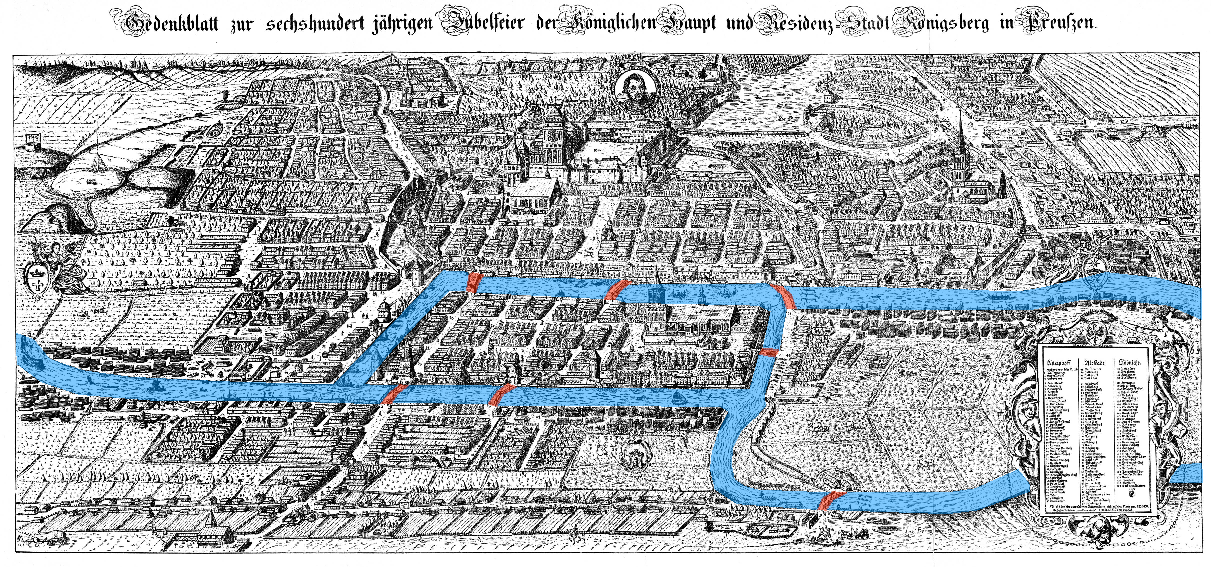
\includegraphics[width=\linewidth]{konigsberg}
\end{figure*}

Dove A,B,C,D sono le quattro zone della città e poi ci sono i vari archi che le connettono, proprio come si vede nell’immagine della città qui sopra.

Ciò che Eulero stava cercando, come molti altri prima di lui,  era un cammino che permettesse di percorrere tutti i ponti esattamente una volta. Provando più e più volte si può vedere come tale risultato non sia raggiungibile.

Ma per fortuna la matematica non è fatta di prove ed errori solamente, ma è fatta di teoremi e risultati generali.

Lui disse e mostrò i due seguenti risultati:

    E’ possibile percorrere tutti gli archi una e una sola volta, concludendo il percorso in un nodo diverso da quello iniziale, se e soltanto se esce un numero dispari di archi soltanto da 2 nodi oppure da nessuno.

Il percorso descritto nelle 3 righe precedenti è detto: Cammino Euleriano

    E’ possibile percorrere tutti gli archi una e una sola volta, concludendo il percorso nel nodo iniziale, se e soltanto se esce un numero pari di archi da tutti i nodi del grafo.

Il percorso qui descritto prende invece il nome di : Ciclo Euleriano.

Chiaramente ciò che stiamo cercando nella città di Konigsberg è un cammino Euleriano. Infatti non abbiamo la pretesa di tornare da dove siamo partiti, ma la necessità di attraversare tutti i ponti una ed una sola volta.

Calcoliamo quindi il grado di tutti e 4 i nodi, dove per grado si intende il numero di archi uscenti dal nodo stesso (in questo caso entranti o uscenti è indifferente dato che non è un grafo orientato).

Il grado di A,B,D è 3, mentre il grado di C è 5. Come si può ben vedere, sono tutti numeri dispari e quindi nessuno tra i due percorsi descritti in precedenza sono presenti nella citta di Konigsberg.

Ecco la risposta alla domanda
Altri due esempi semplici

Devi sapere che l’esistenza di cammini e cicli Euleriani in grafi è esattamente ciò che cercavi da piccolo quando provavi a disegnare una stella o una casetta senza staccare la matita dal foglio!

ponti di Konigsberg

ponti di KoningsbergPoniamoci quindi un paio di domande per descrivere “matematicamente” questi due oggetti che sembrano così semplici. Esiste un solo modo per tracciare tali disegni senza staccare la penna dal foglio? Perchè è possibile disegnarli? Si inizia e finisce il disegno nello stesso punto?

Per rispondere a queste, partiamo dalla casetta. Infatti i due disegni si comportano in modo molto diverso rispetto alle questioni sollevate nelle domande precedenti.

La casetta ha tutti nodi di grado pari, tranne i due nodi alla base. Essi hanno grado dispari: tre. Ecco spigato il motivo per cui sia possibile costruire la casetta senza staccare la penna, infatti tale grafo connesso ammette cammino euleriano, dato che ha esattamente 2 nodi di grado dispari. Ammette però ciclo euleriano? No, per lo stesso motivo, altrimenti dovrebbero essere tutti nodi pari.

Dicendo che esiste un cammino euleriano abbiamo implicitamente detto anche che qualsiasi disegno che ci consenta di tracciare la casetta inizi e finisca in due nodi diversi della casa. Ma resta un’ultima domanda: esiste un solo modo per disegnarla? Beh, in realtà ne esistono due. Infatti il motivo per cui si debbano avere esattamente due nodi dispari per tracciare un cammino euleriano è che l’arco che li rende rispettivamente dispari viene utilizzato per uscire dal nodo iniziale e per entrare nel nodo finale per concludere il disegno.

Prova a pensarci un attimo…se un nodo ha grado pari, ci entro tante volte quante ci esco. Ma nel nodo iniziale io esco una volta in più di quelle che entro, mentre in quello finale entro una volta in più di quelle che esco. Quindi ogni cammino euleriano che posso costruire inizia in un nodo dispari e conclude nell’altro dispari, ecco il perchè della duplicità del cammino euleriano e della possibilità di tracciare la casetta.

Per la stella il discorso è un pelo diverso. Se ci fai caso, infatti, la stella ha tutti i nodi di grado pari. In ogni vertice della stella infatti entrano esattamente due archi. Quindi esiste un ciclo euleriano, ovvero un cammino euleriano che inizia e finisce nello stesso nodo.

Ecco perchè posso tracciare la stella senza staccare la penna dal foglio. Ma ho un solo modo per tracciarla? Beh, in realtà in questo caso possono iniziare da uno qualsiasi dei 5 nodi disponibili. Inoltre posso scegliere il tragitto che più preferisco, infatti il grafo è connesso e tutti i nodi sono di grado pari, quindi comunque scelga ho la certezza di entrare in ogni nodo lo stesso numero di volte che ne uscirò.

Interessante come possa esserci della matematica anche nei giochini che facevi con gli amici alle elementari, vero?

Sulla teoria dei grafi si potrebbe dire ancora davvero molto, ma di sicuro se vedo che piace l’argomento dedicherò a tali tematiche ancora vari articoli. A me piace scoprire nuovi risultati e approfondimenti su questi temi, quindi sarei solo che contento di scriverne ancora

Ti lascio un paio di approfondimenti e riferimenti nel caso ti avessi stimolato almeno un po’ a scoprire il grande mondo dei grafi (o geometria delle posizioni, come Eulero definì questo settore della matematica):

    La matematica dei Social Network: introduzione alla teoria dei grafi 
    Introduction to graph theory
    Graph theory
    Sette ponti di Koningsberg UNIMI: PDF
    Dai ponti di Konigsberg al postino cinese
    I sette ponti di Koningsberg UNITO: PDF

Se vuoi vederti un video ben fatto sull’argomento, ti consiglio questo:

e questo

 

Se invece ti fa piacere rileggerti l’articolo con calma, lo puoi scaricare come PDF cliccando sul bottone qui sotto:
SCARICA IL PDF
Condividi: